\section{utility.h File Reference}
\label{utility_8h}\index{utility.h@{utility.h}}
{\tt \#include $<$iostream$>$}\par
{\tt \#include $<$fstream$>$}\par
{\tt \#include \char`\"{}../../LASS/src/Envelope.h\char`\"{}}\par
{\tt \#include \char`\"{}link\-List.h\char`\"{}}\par
{\tt \#include \char`\"{}filevalue.h\char`\"{}}\par


Include dependency graph for utility.h:\begin{figure}[H]
\begin{center}
\leavevmode
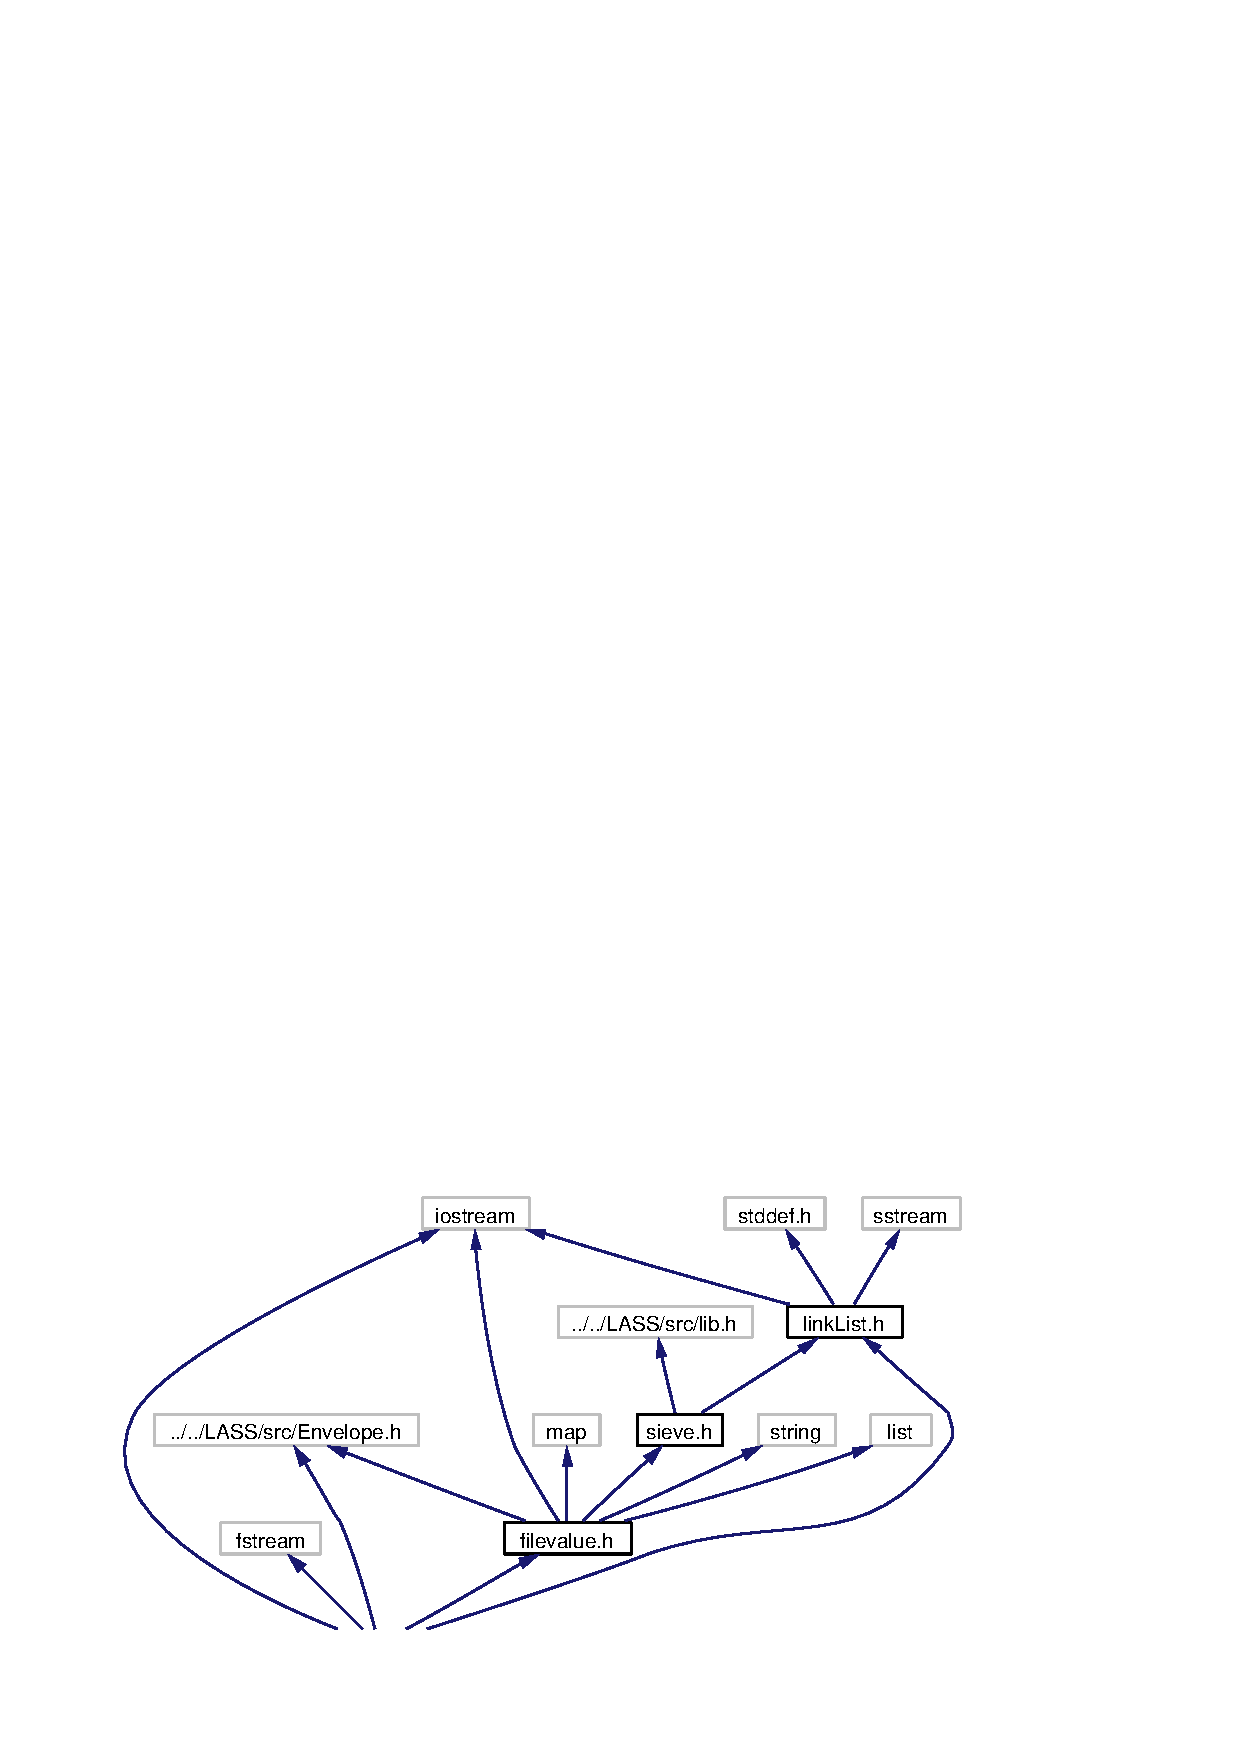
\includegraphics[width=242pt]{utility_8h__incl}
\end{center}
\end{figure}


This graph shows which files directly or indirectly include this file:\begin{figure}[H]
\begin{center}
\leavevmode
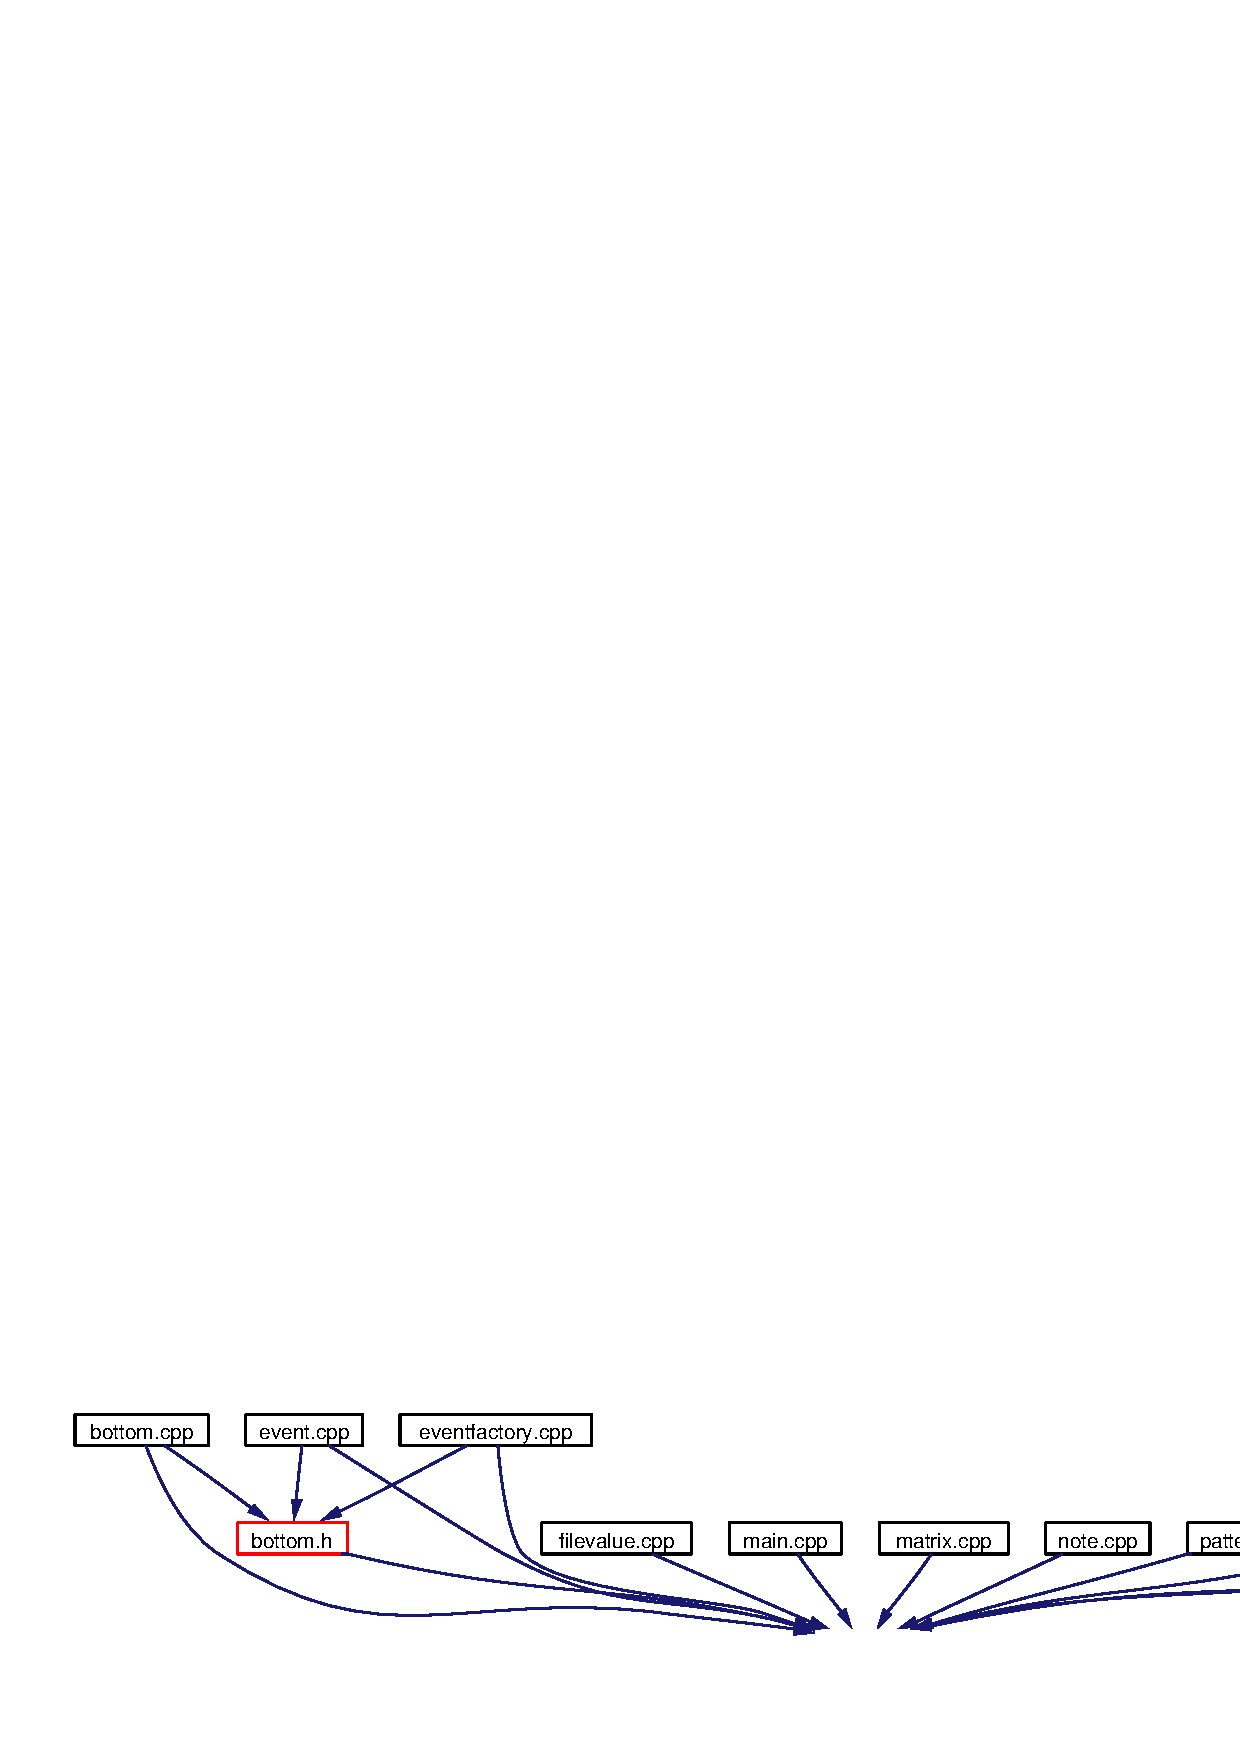
\includegraphics[width=417pt]{utility_8h__dep__incl}
\end{center}
\end{figure}
\subsection*{Functions}
\begin{CompactItemize}
\item 
int {\bf Value\-Pick} (double check\-Point, float abs\-Range)
\item 
int {\bf value\-Pick} (double checkpoint, float abs\-Range, Envelope $\ast$env\-Low, Envelope $\ast$env\-High, Envelope $\ast$env\-Dist, const  char $\ast$e\-Method, vector$<$ int $>$ e\-Arg\-Vect, const  char $\ast$w\-Method, vector$<$ int $>$ w\-Arg\-Vect, const  char $\ast$modify\-Method)
\item 
float {\bf Value\-Float} (double check\-Point, int env\-Num[$\,$], float coef[$\,$])
\item 
float {\bf Value\-Float} (double check\-Point, vector$<$ int $>$ env\-Num, vector$<$ float $>$ coef)
\item 
double {\bf Choose} (double from, double to)
\item 
void {\bf Cumul\-Array} (double array[$\,$], int size)
\item 
void {\bf Cumul\-Weights} ({\bf List}$<$ double $>$ \&a\-List)
\item 
int {\bf Choose\-L} ({\bf List}$<$ double $>$ \&a\-List, {\bf List}$<$ int $>$ \&b\-List)
\item 
float {\bf Stochos} (double check\-Point, int offset)
\item 
float {\bf Stochos} (double check\-Point, int offset, const  char $\ast$method, vector$<$ int $>$ env\-Nums, vector$<$ float $>$ scale)
\item 
float {\bf Stochos} (double check\-Point, int offset, const  char $\ast$method, vector$<$ Envelope $\ast$ $>$ env\-Nums)
\item 
int {\bf Read\-Compute\-Int} (double check\-Point, int offset)
\item 
float {\bf Read\-Compute\-Float} (double check\-Point, int offset)
\item 
void {\bf Non\-Read\-Compute} ()
\item 
string {\bf Read\-Compute\-Chars} (double check\-Point, int offset)
\item 
int {\bf Frequency\-Step} (double check\-Point, int new\-Obj, int type, char $\ast$keep\-Name)
\item 
Envelope $\ast$ {\bf Envelope\-Builder} (char $\ast$method, Collection$<$ xy\_\-point $>$ $\ast$xy\_\-pts, Collection$<$ envelope\_\-segment $>$ $\ast$segs, double check\-Point, int offset, double check, int env\-Num)
\item 
Envelope $\ast$ {\bf Envelope\-Builder} (char $\ast$method, Collection$<$ xy\_\-point $>$ $\ast$xy\_\-pts, Collection$<$ envelope\_\-segment $>$ $\ast$segs, double check\-Point, int offset, double check, int env\-Num, int num\-Segs)
\item 
float {\bf env\-Value} (double check\-Point, int env\-Num, float coef)
\item 
Envelope $\ast$ {\bf Fit\-Envelope} (double check\-Point, int offset)
\item 
Envelope $\ast$ {\bf Select\-Env\-Type} (double check\-Point, int new\-Obj, int type, double check, int offset, char $\ast${\bf file\-Name})
\item 
Envelope $\ast$ {\bf Make\-Envelope} (double check\-Point, int offset, double check)
\item 
Envelope $\ast$ {\bf Segment\-Builder} (double check)
\item 
void {\bf Non\-Env} ()
\item 
int {\bf Choose\-Offset} (int first, int second)
\item 
float {\bf Sequence} (int offset)
\item 
string {\bf Char\-Sequence} (int offset)
\item 
float {\bf Sounds\-Per\-Sec} (float dens)
\item 
float {\bf Sounds\-Per\-Sec} (float dens, int areas, int under\-One)
\item 
void {\bf GSection} ({\bf List}$<$ int $>$ \&a\-List, int levels)
\item 
double {\bf Random\-Source} ()
\item 
double {\bf Rand\-Range} (float low, float high)
\item 
double {\bf Random\-Tri} (float low, float high)
\item 
float {\bf Prefered\-Value\-Distribution} (float value, double check\-Point)
\item 
bool {\bf Chance} (int go\-Flag, double check\-Point, int offset)
\item 
bool {\bf Chance} (double check\-Point, Envelope $\ast$chance\-Env)
\item 
double {\bf Randomizer} ()
\item 
int {\bf Choose\-A} (double probs[$\,$], int size)
\item 
float {\bf Choose\-From\-List} (float array[$\,$], int size)
\item 
void {\bf Flat\-Distribution} ({\bf List}$<$ double $>$ \&a\-Prob\-List)
\item 
int {\bf Random\-Number} (int low\-Num, int high\-Num)
\item 
void {\bf Weights} (double {\bf prob\-Array}[$\,$], int list\-Len)
\item 
void {\bf Clear} (double {\bf prob\-Array}[$\,$], int array\-Size)
\item 
double {\bf Exponential} (int step, double extra)
\item 
float {\bf Sum} (double array[$\,$], int size)
\item 
void {\bf Normalize} (double array[$\,$], int size)
\item 
void {\bf Test\-Library} ()
\item 
void $\ast$ {\bf Evaluate} ({\bf File\-Value} $\ast$value)
\item 
{\bf File\-Value} {\bf Select} (std::list$<$ {\bf File\-Value} $>$ l, int n)
\end{CompactItemize}
\subsection*{Variables}
\begin{CompactItemize}
\item 
double $\ast$ {\bf prob\-Array}
\item 
int {\bf sever}
\end{CompactItemize}


\subsection{Function Documentation}
\index{utility.h@{utility.h}!Chance@{Chance}}
\index{Chance@{Chance}!utility.h@{utility.h}}
\subsubsection{\setlength{\rightskip}{0pt plus 5cm}bool Chance (double {\em check\-Point}, Envelope $\ast$ {\em chance\-Env})}\label{utility_8h_a37}




Definition at line 1558 of file utility.cpp.

References Random::Rand().

Referenced by Bottom::Modifiers(), Bottom::Reverberation(), and Bottom::Spatialization().

Here is the call graph for this function:\begin{figure}[H]
\begin{center}
\leavevmode
\includegraphics[width=109pt]{utility_8h_a37_cgraph}
\end{center}
\end{figure}
\index{utility.h@{utility.h}!Chance@{Chance}}
\index{Chance@{Chance}!utility.h@{utility.h}}
\subsubsection{\setlength{\rightskip}{0pt plus 5cm}bool Chance (int {\em go\-Flag}, double {\em check\-Point}, int {\em offset})}\label{utility_8h_a36}


Returns a value of TRUE or FALSE for the comparison: random\-Number $<$= probability and it is used to force one of these values. The go\-Flag is initialized to 0 for the first time Chance is called. If the probability (which is read in) has the value of -1 ($<$ 0), it is assigned the value of the go\-Flag (either 0 or 1) thus influencing the outcome of the next call. The value of 1 is assigned (in the calling function, not in here) if the comparison was successful (TRUE). If 0 $<$ probability $<$ 1 the outcome depends of the comparison with random\-Number. If the probability $>$ 1 it becomes 0 if go\-Flag = 1, i.e. if a similar param has already been assigned.

In the case of parameters which are dependent of one another, the first (influencing) parameter should have a probability assigned while the subsequent (dependent) parameters should be assigned a value $<$ 0.

In the case of competing aspects of the same parameter (e.g. glissando and detuning) the second one is selected ONLY if the first one was not. \begin{Desc}
\item[Parameters:]
\begin{description}
\item[{\em go\-Flag}]\item[{\em check\-Point}]\item[{\em offset}]\end{description}
\end{Desc}
\begin{Desc}
\item[Returns:]The result of the comparison \end{Desc}


Definition at line 1517 of file utility.cpp.

References Envelope\-Builder(), and Random::Rand().

Here is the call graph for this function:\begin{figure}[H]
\begin{center}
\leavevmode
\includegraphics[width=113pt]{utility_8h_a36_cgraph}
\end{center}
\end{figure}
\index{utility.h@{utility.h}!CharSequence@{CharSequence}}
\index{CharSequence@{CharSequence}!utility.h@{utility.h}}
\subsubsection{\setlength{\rightskip}{0pt plus 5cm}string Char\-Sequence (int {\em offset})}\label{utility_8h_a28}


This function returns the value of the (n)th element in a sequence of chars \begin{Desc}
\item[Parameters:]
\begin{description}
\item[{\em The}]offset to use \end{description}
\end{Desc}
\begin{Desc}
\item[Returns:]The value of the (n)th element \end{Desc}


Definition at line 1350 of file utility.cpp.

References Data\-In::Gen\-Chars(), Data\-In::int\-Vect, Data\-In::name\-Of, and Data\-In::Read\-Ints().

Here is the call graph for this function:\begin{figure}[H]
\begin{center}
\leavevmode
\includegraphics[width=132pt]{utility_8h_a28_cgraph}
\end{center}
\end{figure}
\index{utility.h@{utility.h}!Choose@{Choose}}
\index{Choose@{Choose}!utility.h@{utility.h}}
\subsubsection{\setlength{\rightskip}{0pt plus 5cm}double Choose (double {\em from}, double {\em to})}\label{utility_8h_a6}


This function chooses a random number in the given range (from-to) \begin{Desc}
\item[Parameters:]
\begin{description}
\item[{\em from}]{\bf Bottom}{\rm (p.\,\pageref{classBottom})} of the range \item[{\em to}]{\bf Top}{\rm (p.\,\pageref{classTop})} of the range \end{description}
\end{Desc}


Definition at line 209 of file utility.cpp.

References Random::Rand().

Here is the call graph for this function:\begin{figure}[H]
\begin{center}
\leavevmode
\includegraphics[width=109pt]{utility_8h_a6_cgraph}
\end{center}
\end{figure}
\index{utility.h@{utility.h}!ChooseA@{ChooseA}}
\index{ChooseA@{ChooseA}!utility.h@{utility.h}}
\subsubsection{\setlength{\rightskip}{0pt plus 5cm}int Choose\-A (double {\em probs}[$\,$], int {\em size})}\label{utility_8h_a39}


This function chooses a value out of an array of probabilites \begin{Desc}
\item[Parameters:]
\begin{description}
\item[{\em probs}]The array of probabilites \item[{\em size}]The size of the array \end{description}
\end{Desc}
\begin{Desc}
\item[Returns:]The chosen value \end{Desc}


Definition at line 1607 of file utility.cpp.

References Random::Rand().

Here is the call graph for this function:\begin{figure}[H]
\begin{center}
\leavevmode
\includegraphics[width=113pt]{utility_8h_a39_cgraph}
\end{center}
\end{figure}
\index{utility.h@{utility.h}!ChooseFromList@{ChooseFromList}}
\index{ChooseFromList@{ChooseFromList}!utility.h@{utility.h}}
\subsubsection{\setlength{\rightskip}{0pt plus 5cm}float Choose\-From\-List (float {\em array}[$\,$], int {\em size})}\label{utility_8h_a40}


This function chooses a value from a list of floats. \begin{Desc}
\item[Parameters:]
\begin{description}
\item[{\em array}]The array of floats \item[{\em size}]The size of the array \end{description}
\end{Desc}
\begin{Desc}
\item[Returns:]The chosen value \end{Desc}


Definition at line 1629 of file utility.cpp.

References Random::Rand().

Here is the call graph for this function:\begin{figure}[H]
\begin{center}
\leavevmode
\includegraphics[width=131pt]{utility_8h_a40_cgraph}
\end{center}
\end{figure}
\index{utility.h@{utility.h}!ChooseL@{ChooseL}}
\index{ChooseL@{ChooseL}!utility.h@{utility.h}}
\subsubsection{\setlength{\rightskip}{0pt plus 5cm}int Choose\-L ({\bf List}$<$ double $>$ \& {\em a\-List}, {\bf List}$<$ int $>$ \& {\em b\-List})}\label{utility_8h_a9}


This function chooses an element from a list of integers by matching its probability of occurence stored in a corresponding list of doubles with a random number. \begin{Desc}
\item[Parameters:]
\begin{description}
\item[{\em b\-List}]The list of integers \item[{\em a\-List}]The list of doubles \end{description}
\end{Desc}


Definition at line 272 of file utility.cpp.

References List$<$ Etype $>$::Head(), List$<$ Etype $>$::Length(), Random::Rand(), and List$<$ Etype $>$::Retrieve().

Here is the call graph for this function:\begin{figure}[H]
\begin{center}
\leavevmode
\includegraphics[width=113pt]{utility_8h_a9_cgraph}
\end{center}
\end{figure}
\index{utility.h@{utility.h}!ChooseOffset@{ChooseOffset}}
\index{ChooseOffset@{ChooseOffset}!utility.h@{utility.h}}
\subsubsection{\setlength{\rightskip}{0pt plus 5cm}int Choose\-Offset (int {\em first}, int {\em second})}\label{utility_8h_a26}


This function chooses an appropriate offset based on what is read in. \begin{Desc}
\item[Parameters:]
\begin{description}
\item[{\em first}]This argument is new\-Obj in most cases \item[{\em second}]This argument is type in most cases \end{description}
\end{Desc}
\begin{Desc}
\item[Returns:]The offset \end{Desc}


Definition at line 1295 of file utility.cpp.

Referenced by Event::Continuum3(), Event::Num\-Objs(), Bottom::One\-Step(), and Event::Sweep3().\index{utility.h@{utility.h}!Clear@{Clear}}
\index{Clear@{Clear}!utility.h@{utility.h}}
\subsubsection{\setlength{\rightskip}{0pt plus 5cm}void Clear (double {\em prob\-Array}[$\,$], int {\em array\-Size})}\label{utility_8h_a44}


This function clears the probability array. \begin{Desc}
\item[Parameters:]
\begin{description}
\item[{\em prob\-Array}]The array of probabilites \item[{\em array\-Size}]The size of the array \end{description}
\end{Desc}


Definition at line 1734 of file utility.cpp.

References prob\-Array.\index{utility.h@{utility.h}!CumulArray@{CumulArray}}
\index{CumulArray@{CumulArray}!utility.h@{utility.h}}
\subsubsection{\setlength{\rightskip}{0pt plus 5cm}void Cumul\-Array (double {\em array}[$\,$], int {\em size})}\label{utility_8h_a7}


This function takes an array of doubles, divides each element by the sum of all elements, and adds the value to the preceding value (sum of values) so that the values range from 0 to 1. \begin{Desc}
\item[Parameters:]
\begin{description}
\item[{\em array}]An array of doubles \item[{\em size}]\end{description}
\end{Desc}


Definition at line 226 of file utility.cpp.

References Normalize().

Referenced by Patter::Equivalence().

Here is the call graph for this function:\begin{figure}[H]
\begin{center}
\leavevmode
\includegraphics[width=146pt]{utility_8h_a7_cgraph}
\end{center}
\end{figure}
\index{utility.h@{utility.h}!CumulWeights@{CumulWeights}}
\index{CumulWeights@{CumulWeights}!utility.h@{utility.h}}
\subsubsection{\setlength{\rightskip}{0pt plus 5cm}void Cumul\-Weights ({\bf List}$<$ double $>$ \& {\em a\-List})}\label{utility_8h_a8}


This function takes each weight on the list, divides it by the sum and then adds it to a cumulative weight or probability. \begin{Desc}
\item[Parameters:]
\begin{description}
\item[{\em a\-List}]A list of weights \end{description}
\end{Desc}


Definition at line 247 of file utility.cpp.

References List$<$ Etype $>$::Head(), List$<$ Etype $>$::Length(), List$<$ Etype $>$::Normalize(), List$<$ Etype $>$::Retrieve(), and List$<$ Etype $>$::Update().

Here is the call graph for this function:\begin{figure}[H]
\begin{center}
\leavevmode
\includegraphics[width=228pt]{utility_8h_a8_cgraph}
\end{center}
\end{figure}
\index{utility.h@{utility.h}!EnvelopeBuilder@{EnvelopeBuilder}}
\index{EnvelopeBuilder@{EnvelopeBuilder}!utility.h@{utility.h}}
\subsubsection{\setlength{\rightskip}{0pt plus 5cm}Envelope$\ast$ Envelope\-Builder (char $\ast$ {\em method}, Collection$<$ xy\_\-point $>$ $\ast$ {\em xy\_\-pts}, Collection$<$ envelope\_\-segment $>$ $\ast$ {\em segs}, double {\em check\-Point}, int {\em offset}, double {\em check}, int {\em env\-Num}, int {\em num\-Segs})}\label{utility_8h_a19}


This function serves as a wrapper for the constructors of Envelope from LASS. This combines the previous utility methods of Fit\-Envelope, Select\-Env\-Type, Make\-Envelope, and Segment\-Builder \begin{Desc}
\item[Parameters:]
\begin{description}
\item[{\em method}]A string to determine which method of creating the envelope will be used\-Possible values are: SEG\_\-BUILDER, SEGS\_\-AND\_\-POINTS, FROM\_\-LIB\_\-SCALE, FROM\_\-LIB\_\-NUM \item[{\em xy\_\-pts}]A collection of xy\_\-points \item[{\em segs}]A collection of envelope segements \item[{\em check\-Point}]\item[{\em offset}]\item[{\em check}]\item[{\em env\-Num}]The number of the envelope to load from the library \item[{\em num\-Segs}]The number of segments \end{description}
\end{Desc}
\begin{Desc}
\item[Returns:]An Envelope \end{Desc}
\begin{Desc}
\item[Author:]Chris Ham \end{Desc}


Referenced by Chance(), Bottom::Modifiers(), Bottom::One\-Step(), and Value\-Float().\index{utility.h@{utility.h}!EnvelopeBuilder@{EnvelopeBuilder}}
\index{EnvelopeBuilder@{EnvelopeBuilder}!utility.h@{utility.h}}
\subsubsection{\setlength{\rightskip}{0pt plus 5cm}Envelope$\ast$ Envelope\-Builder (char $\ast$ {\em method}, Collection$<$ xy\_\-point $>$ $\ast$ {\em xy\_\-pts}, Collection$<$ envelope\_\-segment $>$ $\ast$ {\em segs}, double {\em check\-Point}, int {\em offset}, double {\em check}, int {\em env\-Num})}\label{utility_8h_a18}


METHOD: SEGMENT BUILDER /////////////////////////////

METHOD: SEGMENTS AND POINTS /////////////////////////////////

METHOD: LOAD FROM LIBRARY /////////////////////////////////// 

Definition at line 672 of file utility.cpp.

References envlib, Data\-In::file\-Loc(), Data\-In::Gen\-Ints(), Data\-In::g\-Int\-Vect, Read\-Compute\-Chars(), Read\-Compute\-Float(), Read\-Compute\-Int(), and Data\-In::rewind\-File().

Here is the call graph for this function:\begin{figure}[H]
\begin{center}
\leavevmode
\includegraphics[width=145pt]{utility_8h_a18_cgraph}
\end{center}
\end{figure}
\index{utility.h@{utility.h}!envValue@{envValue}}
\index{envValue@{envValue}!utility.h@{utility.h}}
\subsubsection{\setlength{\rightskip}{0pt plus 5cm}float env\-Value (double {\em check\-Point}, int {\em env\-Num}, float {\em coef})}\label{utility_8h_a20}


This function finds the value of an envelope at a given point. The envelope is loaded first (from an Envelope library) and then scaled according to a given coefficient. \begin{Desc}
\item[Parameters:]
\begin{description}
\item[{\em check\-Point}]The point at which to check the envelope \item[{\em env\-Num}]The number of the envelope to load from the library \item[{\em coef}]The coefficient by which to scale the envelope \end{description}
\end{Desc}
\begin{Desc}
\item[Returns:]The value of the envelope at the specified point \end{Desc}
\begin{Desc}
\item[Note:]THIS METHOD WILL SOON BE DEPRECATED. USE Envelope::Get\-Scaled\-Value INSTEAD. \end{Desc}


Definition at line 1024 of file utility.cpp.

References envlib.\index{utility.h@{utility.h}!Evaluate@{Evaluate}}
\index{Evaluate@{Evaluate}!utility.h@{utility.h}}
\subsubsection{\setlength{\rightskip}{0pt plus 5cm}void$\ast$ Evaluate ({\bf File\-Value} $\ast$ {\em value})}\label{utility_8h_a49}




Definition at line 1828 of file utility.cpp.

References File\-Value::get\-Number(), File\-Value::get\-String(), File\-Value::is\-List(), File\-Value::is\-Number(), and File\-Value::is\-String().

Here is the call graph for this function:\begin{figure}[H]
\begin{center}
\leavevmode
\includegraphics[width=130pt]{utility_8h_a49_cgraph}
\end{center}
\end{figure}
\index{utility.h@{utility.h}!Exponential@{Exponential}}
\index{Exponential@{Exponential}!utility.h@{utility.h}}
\subsubsection{\setlength{\rightskip}{0pt plus 5cm}double Exponential (int {\em step}, double {\em extra})}\label{utility_8h_a45}


This function is the inverse exponential function to allow for an extra term (random) deviation. \begin{Desc}
\item[Parameters:]
\begin{description}
\item[{\em step}]\item[{\em extra}]\end{description}
\end{Desc}


Definition at line 1746 of file utility.cpp.

Referenced by Bottom::Rules().\index{utility.h@{utility.h}!FitEnvelope@{FitEnvelope}}
\index{FitEnvelope@{FitEnvelope}!utility.h@{utility.h}}
\subsubsection{\setlength{\rightskip}{0pt plus 5cm}Envelope$\ast$ Fit\-Envelope (double {\em check\-Point}, int {\em offset})}\label{utility_8h_a21}


This function fits (scales) an envelope by a computed coefficient. \begin{Desc}
\item[Parameters:]
\begin{description}
\item[{\em check\-Point}]\item[{\em offset}]\end{description}
\end{Desc}
\begin{Desc}
\item[Returns:]An Envelope \end{Desc}
\begin{Desc}
\item[Note:]THIS METHOD WILL SOON BE DEPRECATED. USE {\bf Envelope::Fit\-Envelope}{\rm (p.\,\pageref{utility_8h_a21})} INSTEAD. \end{Desc}
\index{utility.h@{utility.h}!FlatDistribution@{FlatDistribution}}
\index{FlatDistribution@{FlatDistribution}!utility.h@{utility.h}}
\subsubsection{\setlength{\rightskip}{0pt plus 5cm}void Flat\-Distribution ({\bf List}$<$ double $>$ \& {\em a\-Prob\-List})}\label{utility_8h_a41}


This function assigns even probabilities to a list. \begin{Desc}
\item[Parameters:]
\begin{description}
\item[{\em a\-Problist}]A list of probabilities \end{description}
\end{Desc}
\index{utility.h@{utility.h}!FrequencyStep@{FrequencyStep}}
\index{FrequencyStep@{FrequencyStep}!utility.h@{utility.h}}
\subsubsection{\setlength{\rightskip}{0pt plus 5cm}int Frequency\-Step (double {\em check\-Point}, int {\em new\-Obj}, int {\em type}, char $\ast$ {\em keep\-Name})}\label{utility_8h_a17}


This function is used to find discrete values of a defined tuning \begin{Desc}
\item[Parameters:]
\begin{description}
\item[{\em check\-Point}]\item[{\em new\-Obj}]\item[{\em type}]\item[{\em keep\-Name}]\end{description}
\end{Desc}
\index{utility.h@{utility.h}!GSection@{GSection}}
\index{GSection@{GSection}!utility.h@{utility.h}}
\subsubsection{\setlength{\rightskip}{0pt plus 5cm}void GSection ({\bf List}$<$ int $>$ \& {\em a\-List}, int {\em levels})}\label{utility_8h_a31}


This function partitions a segment into golden mean ratios at multiple levels. \begin{Desc}
\item[Parameters:]
\begin{description}
\item[{\em a\-List}]\item[{\em levels}]\end{description}
\end{Desc}


Definition at line 1420 of file utility.cpp.

References List$<$ Etype $>$::Head(), List$<$ Etype $>$::Insert\-In\-Order(), and List$<$ Etype $>$::Retrieve().

Referenced by Event::Stimes().

Here is the call graph for this function:\begin{figure}[H]
\begin{center}
\leavevmode
\includegraphics[width=184pt]{utility_8h_a31_cgraph}
\end{center}
\end{figure}
\index{utility.h@{utility.h}!MakeEnvelope@{MakeEnvelope}}
\index{MakeEnvelope@{MakeEnvelope}!utility.h@{utility.h}}
\subsubsection{\setlength{\rightskip}{0pt plus 5cm}Envelope$\ast$ Make\-Envelope (double {\em check\-Point}, int {\em offset}, double {\em check})}\label{utility_8h_a23}


This function makes an envelope. \begin{Desc}
\item[Parameters:]
\begin{description}
\item[{\em check\-Point}]\item[{\em offset}]\item[{\em check}]\end{description}
\end{Desc}
\begin{Desc}
\item[Returns:]A pointer to an Envelope \end{Desc}
\begin{Desc}
\item[Note:]THIS METHOD WILL SOON BE DEPRECATED. USE {\bf Utility::Envelope\-Builder}{\rm (p.\,\pageref{utility_8h_a19})} INSTEAD. Use method = SEG\_\-BUILDER with same parameters as here. \end{Desc}
\index{utility.h@{utility.h}!NonEnv@{NonEnv}}
\index{NonEnv@{NonEnv}!utility.h@{utility.h}}
\subsubsection{\setlength{\rightskip}{0pt plus 5cm}void Non\-Env ()}\label{utility_8h_a25}


This function skips a certain number of lines based on the method in the file. \index{utility.h@{utility.h}!NonReadCompute@{NonReadCompute}}
\index{NonReadCompute@{NonReadCompute}!utility.h@{utility.h}}
\subsubsection{\setlength{\rightskip}{0pt plus 5cm}void Non\-Read\-Compute ()}\label{utility_8h_a15}


This function finds out by which method something is determined: by following a sequence, by choosing it from a list, by computing it or by picking a random value. 

Definition at line 534 of file utility.cpp.\index{utility.h@{utility.h}!Normalize@{Normalize}}
\index{Normalize@{Normalize}!utility.h@{utility.h}}
\subsubsection{\setlength{\rightskip}{0pt plus 5cm}void Normalize (double {\em array}[$\,$], int {\em size})}\label{utility_8h_a47}


This function normalizes each element of the array by dividing it by the sum of the array. \begin{Desc}
\item[Parameters:]
\begin{description}
\item[{\em array}]The array \item[{\em size}]The size of the array \end{description}
\end{Desc}


Definition at line 1782 of file utility.cpp.

References Sum().

Referenced by Cumul\-Array(), and Sieve::Cumul\-Array().

Here is the call graph for this function:\begin{figure}[H]
\begin{center}
\leavevmode
\includegraphics[width=91pt]{utility_8h_a47_cgraph}
\end{center}
\end{figure}
\index{utility.h@{utility.h}!PreferedValueDistribution@{PreferedValueDistribution}}
\index{PreferedValueDistribution@{PreferedValueDistribution}!utility.h@{utility.h}}
\subsubsection{\setlength{\rightskip}{0pt plus 5cm}float Prefered\-Value\-Distribution (float {\em value}, double {\em check\-Point})}\label{utility_8h_a35}


This function generates a probability \begin{Desc}
\item[Parameters:]
\begin{description}
\item[{\em value}]\item[{\em check\-Point}]\end{description}
\end{Desc}
\begin{Desc}
\item[Returns:]A probability \end{Desc}


Definition at line 1496 of file utility.cpp.

Referenced by Sieve::Add\-Envelope().\index{utility.h@{utility.h}!Randomizer@{Randomizer}}
\index{Randomizer@{Randomizer}!utility.h@{utility.h}}
\subsubsection{\setlength{\rightskip}{0pt plus 5cm}double Randomizer ()}\label{utility_8h_a38}


This function computes a positive or negative percentage to be added to a value calculated through some other method. \begin{Desc}
\item[Returns:]The positive or negative percentage \end{Desc}
\index{utility.h@{utility.h}!RandomNumber@{RandomNumber}}
\index{RandomNumber@{RandomNumber}!utility.h@{utility.h}}
\subsubsection{\setlength{\rightskip}{0pt plus 5cm}int Random\-Number (int {\em low\-Num}, int {\em high\-Num})\hspace{0.3cm}{\tt  [static]}}\label{utility_8h_a42}


This function returns a random integer between low\-Num and high\-Num. \begin{Desc}
\item[Parameters:]
\begin{description}
\item[{\em low\-Num}]The lower number \item[{\em high\-Num}]The higher number \end{description}
\end{Desc}
\begin{Desc}
\item[Returns:]A random integer between low\-Num and high\-Num \end{Desc}
\index{utility.h@{utility.h}!RandomSource@{RandomSource}}
\index{RandomSource@{RandomSource}!utility.h@{utility.h}}
\subsubsection{\setlength{\rightskip}{0pt plus 5cm}double Random\-Source ()}\label{utility_8h_a32}


This function is a generic method for generating random numbers between 0 and 1 using a flat distribution. \begin{Desc}
\item[Returns:]A random number between 0 and 1 \end{Desc}
\index{utility.h@{utility.h}!RandomTri@{RandomTri}}
\index{RandomTri@{RandomTri}!utility.h@{utility.h}}
\subsubsection{\setlength{\rightskip}{0pt plus 5cm}double Random\-Tri (float {\em low}, float {\em high})}\label{utility_8h_a34}


This function generates a random number with a triangular distribution \begin{Desc}
\item[Parameters:]
\begin{description}
\item[{\em low}]The minimum of the range \item[{\em high}]The maximum of the range \end{description}
\end{Desc}
\begin{Desc}
\item[Returns:]A random number within the specified range \end{Desc}
\index{utility.h@{utility.h}!RandRange@{RandRange}}
\index{RandRange@{RandRange}!utility.h@{utility.h}}
\subsubsection{\setlength{\rightskip}{0pt plus 5cm}double Rand\-Range (float {\em low}, float {\em high})}\label{utility_8h_a33}


This function generates a random number within a range (low to high) using a flat distribution. \begin{Desc}
\item[Parameters:]
\begin{description}
\item[{\em low}]The minimum of the range \item[{\em high}]The maximum of the range \end{description}
\end{Desc}
\begin{Desc}
\item[Returns:]A random number within the specified range \end{Desc}
\index{utility.h@{utility.h}!ReadComputeChars@{ReadComputeChars}}
\index{ReadComputeChars@{ReadComputeChars}!utility.h@{utility.h}}
\subsubsection{\setlength{\rightskip}{0pt plus 5cm}string Read\-Compute\-Chars (double {\em check\-Point}, int {\em offset})}\label{utility_8h_a16}


This function finds out by which method a character value is determined: by reading it, by following a equence, by computing it using Value\-Pick, or by picking a random value within a given range. \begin{Desc}
\item[Parameters:]
\begin{description}
\item[{\em check\-Point}]\item[{\em offset}]\end{description}
\end{Desc}


Definition at line 563 of file utility.cpp.

Referenced by Envelope\-Builder().\index{utility.h@{utility.h}!ReadComputeFloat@{ReadComputeFloat}}
\index{ReadComputeFloat@{ReadComputeFloat}!utility.h@{utility.h}}
\subsubsection{\setlength{\rightskip}{0pt plus 5cm}float Read\-Compute\-Float (double {\em check\-Point}, int {\em offset})}\label{utility_8h_a14}


This function finds out by which method a float value is determined: by following a sequence, by computing it using Stochos, or by picking a random value within a given range. \begin{Desc}
\item[Parameters:]
\begin{description}
\item[{\em check\-Point}]\item[{\em offset}]\end{description}
\end{Desc}


Definition at line 496 of file utility.cpp.

Referenced by Patter::Chooser(), Event::Continuum3(), Envelope\-Builder(), Event::Num\-Objs(), and Event::Sweep3().\index{utility.h@{utility.h}!ReadComputeInt@{ReadComputeInt}}
\index{ReadComputeInt@{ReadComputeInt}!utility.h@{utility.h}}
\subsubsection{\setlength{\rightskip}{0pt plus 5cm}int Read\-Compute\-Int (double {\em check\-Point}, int {\em offset})}\label{utility_8h_a13}


This function finds out by which method an integer value is determined: by reading it, by following a sequence, by computing it using Value\-Pick, or by picking a random value within a given range. \begin{Desc}
\item[Parameters:]
\begin{description}
\item[{\em check\-Point}]\item[{\em offset}]\end{description}
\end{Desc}


Definition at line 458 of file utility.cpp.

Referenced by Event::Continuum3(), Envelope\-Builder(), Bottom::Modifiers(), Event::Num\-Objs(), and Event::Sweep3().\index{utility.h@{utility.h}!SegmentBuilder@{SegmentBuilder}}
\index{SegmentBuilder@{SegmentBuilder}!utility.h@{utility.h}}
\subsubsection{\setlength{\rightskip}{0pt plus 5cm}Envelope$\ast$ Segment\-Builder (double {\em check})}\label{utility_8h_a24}


This function builds an envelope from scratch by creating a colllection of points (x,y) and a collection of segments. The xy collection is created with Read\-Compute\-Float calling Sequence; instead of the usual double check\-Point showing the point in time when the selection is made, the variable check (double) is used to indicate the position of this particular envelope between the rest of the enveloopes (as a ); the second parameter is the segment number. The file location is remembered and we return to it at the end of the loop to take care of the next segment, build from the same data. \begin{Desc}
\item[Parameters:]
\begin{description}
\item[{\em check}]\end{description}
\end{Desc}
\begin{Desc}
\item[Returns:]A pointer to an Envelope \end{Desc}
\begin{Desc}
\item[Note:]THIS METHOD WILL SOON BE DEPRECATED. USE {\bf Utility::Envelope\-Builder}{\rm (p.\,\pageref{utility_8h_a19})} INSTEAD. Use method = SEG\_\-BUILDER with same parameters as here. \end{Desc}
\index{utility.h@{utility.h}!Select@{Select}}
\index{Select@{Select}!utility.h@{utility.h}}
\subsubsection{\setlength{\rightskip}{0pt plus 5cm}{\bf File\-Value} Select (std::list$<$ {\bf File\-Value} $>$ {\em l}, int {\em n})}\label{utility_8h_a50}




Definition at line 1856 of file utility.cpp.

Referenced by Note::Assign\-Loudness(), Note::Assign\-Pitch(), and File\-Value::Evaluate().\index{utility.h@{utility.h}!SelectEnvType@{SelectEnvType}}
\index{SelectEnvType@{SelectEnvType}!utility.h@{utility.h}}
\subsubsection{\setlength{\rightskip}{0pt plus 5cm}Envelope$\ast$ Select\-Env\-Type (double {\em check\-Point}, int {\em new\-Obj}, int {\em type}, double {\em check}, int {\em offset}, char $\ast$ {\em file\-Name})}\label{utility_8h_a22}


This function creates an envelope based on the given method. \begin{Desc}
\item[Parameters:]
\begin{description}
\item[{\em check\-Point}]\item[{\em new\-Obj}]\item[{\em type}]\item[{\em check}]\item[{\em offset}]\item[{\em file\-Name}]\end{description}
\end{Desc}
\begin{Desc}
\item[Returns:]A pointer to an Envelope \end{Desc}
\begin{Desc}
\item[Note:]THIS METHOD WILL SOON BE DEPRECATED. USE {\bf Utility::Envelope\-Builder}{\rm (p.\,\pageref{utility_8h_a19})} INSTEAD. Use method = SEG\_\-BUILDER -OR- FROM\_\-LIBRARY \end{Desc}
\index{utility.h@{utility.h}!Sequence@{Sequence}}
\index{Sequence@{Sequence}!utility.h@{utility.h}}
\subsubsection{\setlength{\rightskip}{0pt plus 5cm}float Sequence (int {\em offset})}\label{utility_8h_a27}


This function returns the value of the (n)th element in a sequence of floats \begin{Desc}
\item[Parameters:]
\begin{description}
\item[{\em The}]offset to use \end{description}
\end{Desc}
\begin{Desc}
\item[Returns:]The value of the (n)th element \end{Desc}


Definition at line 1330 of file utility.cpp.

References Data\-In::Gen\-Floats(), Data\-In::g\-Float\-Vect, Data\-In::int\-Vect, and Data\-In::Read\-Ints().

Referenced by Bottom::Three\-Step().

Here is the call graph for this function:\begin{figure}[H]
\begin{center}
\leavevmode
\includegraphics[width=120pt]{utility_8h_a27_cgraph}
\end{center}
\end{figure}
\index{utility.h@{utility.h}!SoundsPerSec@{SoundsPerSec}}
\index{SoundsPerSec@{SoundsPerSec}!utility.h@{utility.h}}
\subsubsection{\setlength{\rightskip}{0pt plus 5cm}float Sounds\-Per\-Sec (float {\em dens}, int {\em areas}, int {\em under\-One})}\label{utility_8h_a30}




Definition at line 1401 of file utility.cpp.

Referenced by Event::New\-Num\-Objs(), and Event::Num\-Objs().\index{utility.h@{utility.h}!SoundsPerSec@{SoundsPerSec}}
\index{SoundsPerSec@{SoundsPerSec}!utility.h@{utility.h}}
\subsubsection{\setlength{\rightskip}{0pt plus 5cm}float Sounds\-Per\-Sec (float {\em dens})}\label{utility_8h_a29}


This function maps an \char`\"{}abstract\char`\"{} density of 0 - 1 onto a number of sounds per second by defining a total number of regions (areas) and the number of such areas with less than 1 sound/sec. (under\-One). A common example:

areas 0 1 2 3 4 5 6 7 dens. 0.00 0.125 0.250 0.375 0.500 0.625 0.750 0.875 1.00 s/sec 1/16 1/8 1/4 1/2 1 2 4 8 16

Here, there are 8 areas (0-7) and 4 of them (0-3) include values of less than 1 sound/sec. By subtracting under\-One, a dens = 0 is mapped onto a value of 1 sound every 16 sec. and not onto 0.

In most cases areas = 8 and under\-One = 4 like in the above example. \begin{Desc}
\item[Parameters:]
\begin{description}
\item[{\em dens}]The density \end{description}
\end{Desc}
\begin{Desc}
\item[Returns:]Number of sounds per second \end{Desc}


Definition at line 1372 of file utility.cpp.\index{utility.h@{utility.h}!Stochos@{Stochos}}
\index{Stochos@{Stochos}!utility.h@{utility.h}}
\subsubsection{\setlength{\rightskip}{0pt plus 5cm}float Stochos (double {\em check\-Point}, int {\em offset}, const char $\ast$ {\em method}, vector$<$ Envelope $\ast$ $>$ {\em env\-Nums})}\label{utility_8h_a12}




Definition at line 385 of file utility.cpp.

References Random::Rand().

Referenced by File\-Value::Evaluate().

Here is the call graph for this function:\begin{figure}[H]
\begin{center}
\leavevmode
\includegraphics[width=109pt]{utility_8h_a12_cgraph}
\end{center}
\end{figure}
\index{utility.h@{utility.h}!Stochos@{Stochos}}
\index{Stochos@{Stochos}!utility.h@{utility.h}}
\subsubsection{\setlength{\rightskip}{0pt plus 5cm}float Stochos (double {\em check\-Point}, int {\em offset}, const char $\ast$ {\em method}, vector$<$ int $>$ {\em env\-Nums}, vector$<$ float $>$ {\em scale})}\label{utility_8h_a11}


\index{utility.h@{utility.h}!Stochos@{Stochos}}
\index{Stochos@{Stochos}!utility.h@{utility.h}}
\subsubsection{\setlength{\rightskip}{0pt plus 5cm}float Stochos (double {\em check\-Point}, int {\em offset})}\label{utility_8h_a10}


Stochos. Reads 3 envelope numbers and 3 scaling factors and chooses a value using utility methods Value\-Float and env\-Value. The \char`\"{}offset\char`\"{} points to the triplet needed at this moment given that there might be more than one type of elemets to be considered (such as 2,3,5 etc. types in a layer). \begin{Desc}
\item[Parameters:]
\begin{description}
\item[{\em check\-Point}]\item[{\em offset}]\end{description}
\end{Desc}
\index{utility.h@{utility.h}!Sum@{Sum}}
\index{Sum@{Sum}!utility.h@{utility.h}}
\subsubsection{\setlength{\rightskip}{0pt plus 5cm}float Sum (double {\em array}[$\,$], int {\em size})}\label{utility_8h_a46}


This function calculates the sum of the elements of the array. \begin{Desc}
\item[Parameters:]
\begin{description}
\item[{\em array}]The array \item[{\em size}]The size of the array \end{description}
\end{Desc}


Definition at line 1763 of file utility.cpp.

Referenced by Normalize().\index{utility.h@{utility.h}!TestLibrary@{TestLibrary}}
\index{TestLibrary@{TestLibrary}!utility.h@{utility.h}}
\subsubsection{\setlength{\rightskip}{0pt plus 5cm}void Test\-Library ()}\label{utility_8h_a48}


This function is used for testing purposes. 

Definition at line 1798 of file utility.cpp.

References envlib, and sever.\index{utility.h@{utility.h}!ValueFloat@{ValueFloat}}
\index{ValueFloat@{ValueFloat}!utility.h@{utility.h}}
\subsubsection{\setlength{\rightskip}{0pt plus 5cm}float Value\-Float (double {\em check\-Point}, vector$<$ int $>$ {\em env\-Num}, vector$<$ float $>$ {\em coef})}\label{utility_8h_a5}




Definition at line 169 of file utility.cpp.

References Envelope\-Builder(), and Random::Rand().

Here is the call graph for this function:\begin{figure}[H]
\begin{center}
\leavevmode
\includegraphics[width=122pt]{utility_8h_a5_cgraph}
\end{center}
\end{figure}
\index{utility.h@{utility.h}!ValueFloat@{ValueFloat}}
\index{ValueFloat@{ValueFloat}!utility.h@{utility.h}}
\subsubsection{\setlength{\rightskip}{0pt plus 5cm}float Value\-Float (double {\em check\-Point}, int {\em env\-Num}[$\,$], float {\em coef}[$\,$])}\label{utility_8h_a4}


This function assigns a float value to a parameter. It uses three envelopes and three scale factors: two to find the min and max values at a given time (check\-Point) and the third ones to define a distribution over this range. \begin{Desc}
\item[Parameters:]
\begin{description}
\item[{\em check\-Point}]The given time \item[{\em env\-Num}]An array of envelope numbers \item[{\em coef}]An array of coefficients by which to scale the envelope \end{description}
\end{Desc}


Definition at line 133 of file utility.cpp.

References Envelope\-Builder(), and Random::Rand().

Here is the call graph for this function:\begin{figure}[H]
\begin{center}
\leavevmode
\includegraphics[width=122pt]{utility_8h_a4_cgraph}
\end{center}
\end{figure}
\index{utility.h@{utility.h}!valuePick@{valuePick}}
\index{valuePick@{valuePick}!utility.h@{utility.h}}
\subsubsection{\setlength{\rightskip}{0pt plus 5cm}int value\-Pick (double {\em checkpoint}, float {\em abs\-Range}, Envelope $\ast$ {\em env\-Low}, Envelope $\ast$ {\em env\-High}, Envelope $\ast$ {\em env\-Dist}, const char $\ast$ {\em e\-Method}, vector$<$ int $>$ {\em e\-Arg\-Vect}, const char $\ast$ {\em w\-Method}, vector$<$ int $>$ {\em w\-Arg\-Vect}, const char $\ast$ {\em modify\-Method})}\label{utility_8h_a3}




Definition at line 103 of file utility.cpp.

References Sieve::Build(), and Sieve::Modify().

Referenced by File\-Value::Evaluate().

Here is the call graph for this function:\begin{figure}[H]
\begin{center}
\leavevmode
\includegraphics[width=111pt]{utility_8h_a3_cgraph}
\end{center}
\end{figure}
\index{utility.h@{utility.h}!ValuePick@{ValuePick}}
\index{ValuePick@{ValuePick}!utility.h@{utility.h}}
\subsubsection{\setlength{\rightskip}{0pt plus 5cm}int Value\-Pick (double {\em check\-Point}, float {\em abs\-Range})}\label{utility_8h_a2}


This function finds the lower and upper limits for a set of values at a given time (check\-Point). This is done by finding the values of envelopes for the min and max limits at the check\-Point. Builds a list of possible values within this range and assigns probabilities to them according to both a sieve and another envelope. Picks a value off a list of possible values (elements) by matching its weight or probability to a random number. \begin{Desc}
\item[Parameters:]
\begin{description}
\item[{\em check\-Point}]The given time \item[{\em abs\-Range}]\end{description}
\end{Desc}
\begin{Desc}
\item[Returns:]A value from the list of possible values \end{Desc}


Definition at line 58 of file utility.cpp.

Referenced by Event::Sweep3(), and Bottom::Three\-Step().\index{utility.h@{utility.h}!Weights@{Weights}}
\index{Weights@{Weights}!utility.h@{utility.h}}
\subsubsection{\setlength{\rightskip}{0pt plus 5cm}void Weights (double {\em prob\-Array}[$\,$], int {\em list\-Len})}\label{utility_8h_a43}


This function assigns probabilities according to a list provided by the user.

The HIERARCHIC option adds the weights associated with individual moduli to the same sieve element. Thus, the same element (eg. attack point) can have a weight which is the sum of a number of moduli, each with its own weight (probability).

The PERIODIC option cycles through the available weights creating a meter- like pattern. \begin{Desc}
\item[Parameters:]
\begin{description}
\item[{\em prob\-Array}]An array of probabilities \item[{\em list\-Len}]The length of the list \end{description}
\end{Desc}


\subsection{Variable Documentation}
\index{utility.h@{utility.h}!probArray@{probArray}}
\index{probArray@{probArray}!utility.h@{utility.h}}
\subsubsection{\setlength{\rightskip}{0pt plus 5cm}double$\ast$ {\bf prob\-Array}}\label{utility_8h_a0}




Definition at line 450 of file utility.h.

Referenced by Clear().\index{utility.h@{utility.h}!sever@{sever}}
\index{sever@{sever}!utility.h@{utility.h}}
\subsubsection{\setlength{\rightskip}{0pt plus 5cm}int {\bf sever}}\label{utility_8h_a1}




Definition at line 490 of file utility.h.

Referenced by Patter::Adjust(), Event::Build\-Sub\-Events(), Patter::Chooser(), Patter::Delivery(), Patter::Distort(), Event::Duration\-Methods(), Sieve::Elements(), File\-Value::Evaluate(), Patter::Expand(), Event::New\-Attack\-Methods(), Event::New\-Duration\-Methods(), Event::New\-Num\-Objs(), Event::Num\-Objs(), Bottom::Num\-Part(), Patter::Nursery(), Event::Points\-Probs(), Bottom::Rules(), Bottom::Spatialization(), Bottom::Spectrum(), Event::Sweep3(), Patter::Symmetries(), Test\-Library(), Event::Test\-Name\-Type(), Bottom::Three\-Step(), and Sieve::Weights().